\documentclass[a4paper, 11pt]{article}
\usepackage[hmargin=1in]{geometry}
\usepackage[utf8]{inputenc}
\usepackage[T1, T2A]{fontenc}
\usepackage{csquotes}
\usepackage[main=bulgarian, english]{babel}
\usepackage{amsmath}
\usepackage{amssymb}
\usepackage{amsthm}
\usepackage{listings}
\usepackage{graphicx}
\usepackage{float}
\usepackage{svg}
\usepackage{tikz}
\usepackage{helvet}
\usetikzlibrary{decorations.markings,decorations.shapes,decorations,arrows,automata,backgrounds,petri,shapes.geometric}
\usepackage{xcolor}
\usepackage[style=numeric, sorting=none, language=auto]{biblatex}

\addbibresource{sources.bib}
\allowdisplaybreaks

\begin{document}
\author{Даниел Халачев, ИИОЗ, 4MI3400603}
\title{Онтология на основните стилове в изобразителното изкуство и техните отличителни картини}
\maketitle

\section*{Атомарни концепти}
\begin{itemize}
  \item \textbf{Artwork} - произведение на изкуството
  \item \textbf{Age} - епоха в човешкото развитие
  \item \textbf{Style} - стил в изобразителното изкуство
  \item \textbf{Artist} - художник, нарисувал картината
  \item \textbf{Region} - регион на света, където е работил художникът
  \item \textbf{Medium} - средство за изобразяване
  \item \textbf{Depiction} - какво изобразява картината
  \item \textbf{Museum} - музей, в който се помещава картината днес
\end{itemize}

\section*{Атомарни подконцепти}
\begin{align*}
  &\text{Paint} \sqsubseteq \text{Medium} \\
  &\text{Landscape} \sqsubseteq \text{Depiction}
\end{align*}

\section*{Неатомарни концепти}
\begin{align*}
  \text{Painting} &\doteq \text{[AND Artwork, [EXISTS 1 :depicts], [EXISTS 1 :hasMedium]]} \\
  \text{OilPainting} &\doteq \text{[AND Painting, [FILLS :hasMedium, OilPaint]]} \\
  \text{AcrylicPainting} &\doteq \text{[AND Painting, [FILLS :hasMedium, AcrylicPaint]]} \\
  \text{HistoricalEventPainting} &\doteq \text{[AND Painting, [FILLS :depicts, HistoricalEvent]]} \\
  \text{PortraitPainting} &\doteq \text{[AND Painting, [FILLS :depicts, Portrait]]} \\
  \text{LandscapePainting} &\doteq \text{[AND Painting, [ALL :depicts, Landscape]]} \\
  \text{PortraitOilPainting} &\doteq \text{[AND OilPainting, PortraitPainting]}
\end{align*}

\section*{Роли}
\begin{align*}
  \text{belongsTo} &: \text{Style} \to \text{Age}\\
  \text{represents} &: \text{Artwork} \to \text{Style}\\
  \text{createdBy} &: \text{Artwork} \to \text{Artist}\\
  \text{housedIn} &: \text{Artwork} \to \text{Museum}\\
  \text{locatedIn} &: \text{Museum} \to \text{Region}\\
  \text{negativeReactionTo} &: \text{Style} \to \text{Style}\\
  \text{positiveReactionTo} &: \text{Style} \to \text{Style}\\
  \text{depicts} &: \text{Painting} \to \text{Depiction}\\
  \text{usesMedium} &: \text{Painting} \to \text{Medium}\\
  \text{livedIn} &: \text{Artist} \to \text{Region}\\
  \text{precededBy} &: \text{Age} \to \text{Age}\\
  \text{succeededBy} &: \text{Age} \to \text{Age}.
\end{align*}
\begin{align*}
  &\text{belongsTo}(Paleolithic, PrehistoricAge)\\\\
  &\text{belongsTo}(Neolithic, PrehistoricAge)\\\\
  &\text{belongsTo}(AncientEgyptian, Antiquity)\\\\
  &\text{belongsTo}(AncientGreek, Antiquity) \\
  &\text{positiveReactionTo}(AncientGreek, AncientEgyptian)\\\\
  &\text{belongsTo}(Roman, Antiquity) \\
  &\text{positiveReactionTo}(Roman, AncientGreek)\\\\
  &\text{belongsTo}(Byzantine, MiddleAges)\\\\
  &\text{belongsTo}(Romanesque, MiddleAges)\\\\
  &\text{belongsTo}(Gothic, GothicAge) \\
  &\text{positiveReactionTo}(Gothic, Romanesque)\\\\
  &\text{belongsTo}(ItalianRenaissance, Renaissance) \\
  &\text{negativeReactionTo}(ItalianRenaissance, Gothic)\\\\
  &\text{belongsTo}(NordicRenaissance, Renaissance)\\\\
  &\text{belongsTo}(Baroque, NewAge) \\
  &\text{negativeReactionTo}(Baroque, Renaissance)\\\\
  &\text{belongsTo}(Rococo, NewAge) \\
  &\text{negativeReactionTo}(Rococo, Baroque)\\\\
  &\text{belongsTo}(Classicism, NewAge) \\
  &\text{negativeReactionTo}(Classicism, Rococo)\\\\
  &\text{belongsTo}(Romanticism, NewAge) \\
  &\text{belongsTo}(Realism, ModernAge) \\
  &\text{negativeReactionTo}(Realism, Romanticism)\\\\
  &\text{belongsTo}(Impressionism, ModernAge) \\
  &\text{negativeReactionTo}(Impressionism, Realism)\\\\
  &\text{belongsTo}(PostImpressionism, ModernAge) \\
  &\text{positiveReactionTo}(PostImpressionism, Impressionism)\\\\
  &\text{belongsTo}(Expressionism, ModernAge) \\
  &\text{negativeReactionTo}(Expressionism, Realism)\\\\
  &\text{belongsTo}(Cubism, ModernAge) \\
  &\text{negativeReactionTo}(Cubism, Impressionism)\\\\
  &\text{belongsTo}(Futurism, ModernAge)\\\\
  &\text{belongsTo}(Dadaism, ModernAge)\\\\
  &\text{belongsTo}(Surrealism, ModernAge) \\
  &\text{positiveReactionTo}(Surrealism, Dadaism)\\\\
  &\text{belongsTo}(PopArt, ContemporaryAge) \\\\
  &\text{belongsTo}(ConceptualArt, ContemporaryAge) \\
  &\text{positiveReactionTo}(ConceptualArt, PopArt) \\\\
  &\text{precededBy}(Antiquity, PrehistoricAge) \\
  &\text{succeededBy}(Antiquity, MiddleAges) \\
  &\text{precededBy}(MiddleAges, Antiquity) \\
  &\text{succeededBy}(MiddleAges, GothicAge) \\
  &\text{precededBy}(GothicAge, MiddleAges) \\
  &\text{succeededBy}(GothicAge, Renaissance) \\
  &\text{precededBy}(Renaissance, GothicAge) \\
  &\text{succeededBy}(Renaissance, NewAge) \\
  &\text{precededBy}(NewAge, Renaissance) \\
  &\text{succeededBy}(NewAge, ModernAge) \\
  &\text{precededBy}(ModernAge, NewAge) \\
  &\text{succeededBy}(ModernAge, ContemporaryAge) \\
  &\text{precededBy}(ContemporaryAge, ModernAge)
\end{align*}

От тях \emph{precededBy} и \emph{succeededBy} са противоположни и транзитивни, а \emph{createdBy} и \emph{housedIn} са функционални.

\section*{Константи}
\begin{itemize}
  \item \textbf{Artwork}
    \begin{align*}
      \text{Michelangelo} &\to \text{Artist}\\
      \text{David} &\to \text{Artwork}
    \end{align*}
    \begin{align*}
      &livedIn(Michelangelo, WesternEurope)\\
      &createdBy(David, Michelangelo)\\
      &represents(David, ItalianRenaissance)\\
      &housedIn(David, GalleriaDellAccademia)
    \end{align*}

  \item \textbf{Age}
    \begin{align*}
      \text{PrehistoricAge} &\to \text{Age}\\
      \text{Antiquity} &\to \text{Age}\\
      \text{MiddleAges} &\to \text{Age}\\
      \text{GothicAge} &\to \text{Age}\\
      \text{Renaissance} &\to \text{Age}\\
      \text{NewAge} &\to \text{Age}\\
      \text{ModernAge} &\to \text{Age}\\
      \text{ContemporaryAge} &\to \text{Age}
    \end{align*}
  \item \textbf{Style}
    \begin{align*}
      \text{Paleolithic} &\to \text{Style}\\
      \text{Neolithic} &\to \text{Style}\\
      \text{AncientEgyptian} &\to \text{Style}\\
      \text{AncientGreek} &\to \text{Style}\\
      \text{Roman} &\to \text{Style}\\
      \text{Byzantine} &\to \text{Style}\\
      \text{Romanesque} &\to \text{Style}\\
      \text{Gothic} &\to \text{Style}\\
      \text{ItalianRenaissance} &\to \text{Style}\\
      \text{NordicRenaissance} &\to \text{Style}\\
      \text{Baroque} &\to \text{Style}\\
      \text{Rococo} &\to \text{Style}\\
      \text{Classicism} &\to \text{Style}\\
      \text{Romanticism} &\to \text{Style}\\
      \text{Realism} &\to \text{Style}\\
      \text{Impressionism} &\to \text{Style}\\
      \text{PostImpressionism} &\to \text{Style}\\
      \text{Expressionism} &\to \text{Style}\\
      \text{Cubism} &\to \text{Style}\\
      \text{Futurism} &\to \text{Style}\\
      \text{Dadaism} &\to \text{Style}\\
      \text{Surrealism} &\to \text{Style}\\
      \text{PopArt} &\to \text{Style}\\
      \text{ConceptualArt} &\to \text{Style}
    \end{align*}
  \item \textbf{Medium}
    \begin{align*}
      \text{Chalk} &\to \text{Medium}\\
      \text{Graphite} &\to \text{Medium}
    \end{align*}
  \item \textbf{Paint} $\sqsubseteq$ Medium
    \begin{align*}
      \text{OilPaint} &\to \text{Paint}\\
      \text{AcrylicPaint} &\to \text{Paint}
    \end{align*}
  \item \textbf{Depiction}
    \begin{align*}
      \text{HistoricalEvent} &\to \text{Depiction}\\
      \text{Portrait} &\to \text{Depiction}\\
      \text{GroupScene} &\to \text{Depiction}\\
      \text{AbstractDepiction} &\to \text{Depiction}
    \end{align*}
  \item \textbf{Landscape} $\sqsubseteq$ Depiction
    \begin{align*}
      \text{NaturalLandscape} &\to \text{Landscape}\\
      \text{UrbanLandscape} &\to \text{Landscape}
    \end{align*}
  \item \textbf{Region}
    \begin{align*}
      \text{Asia} &\to \text{Region}\\
      \text{Africa} &\to \text{Region}\\
      \text{Australia} &\to \text{Region}\\
      \text{NorthAmerica} &\to \text{Region}\\
      \text{SouthAmerica} &\to \text{Region}\\
      \text{EasternEurope} &\to \text{Region}\\
      \text{WesternEurope} &\to \text{Region}
    \end{align*}
\end{itemize}
\section*{Визуализация}
\begin{figure}[H]
  \centering
  % \includesvg[width=\linewidth]{images/onto.svg}
  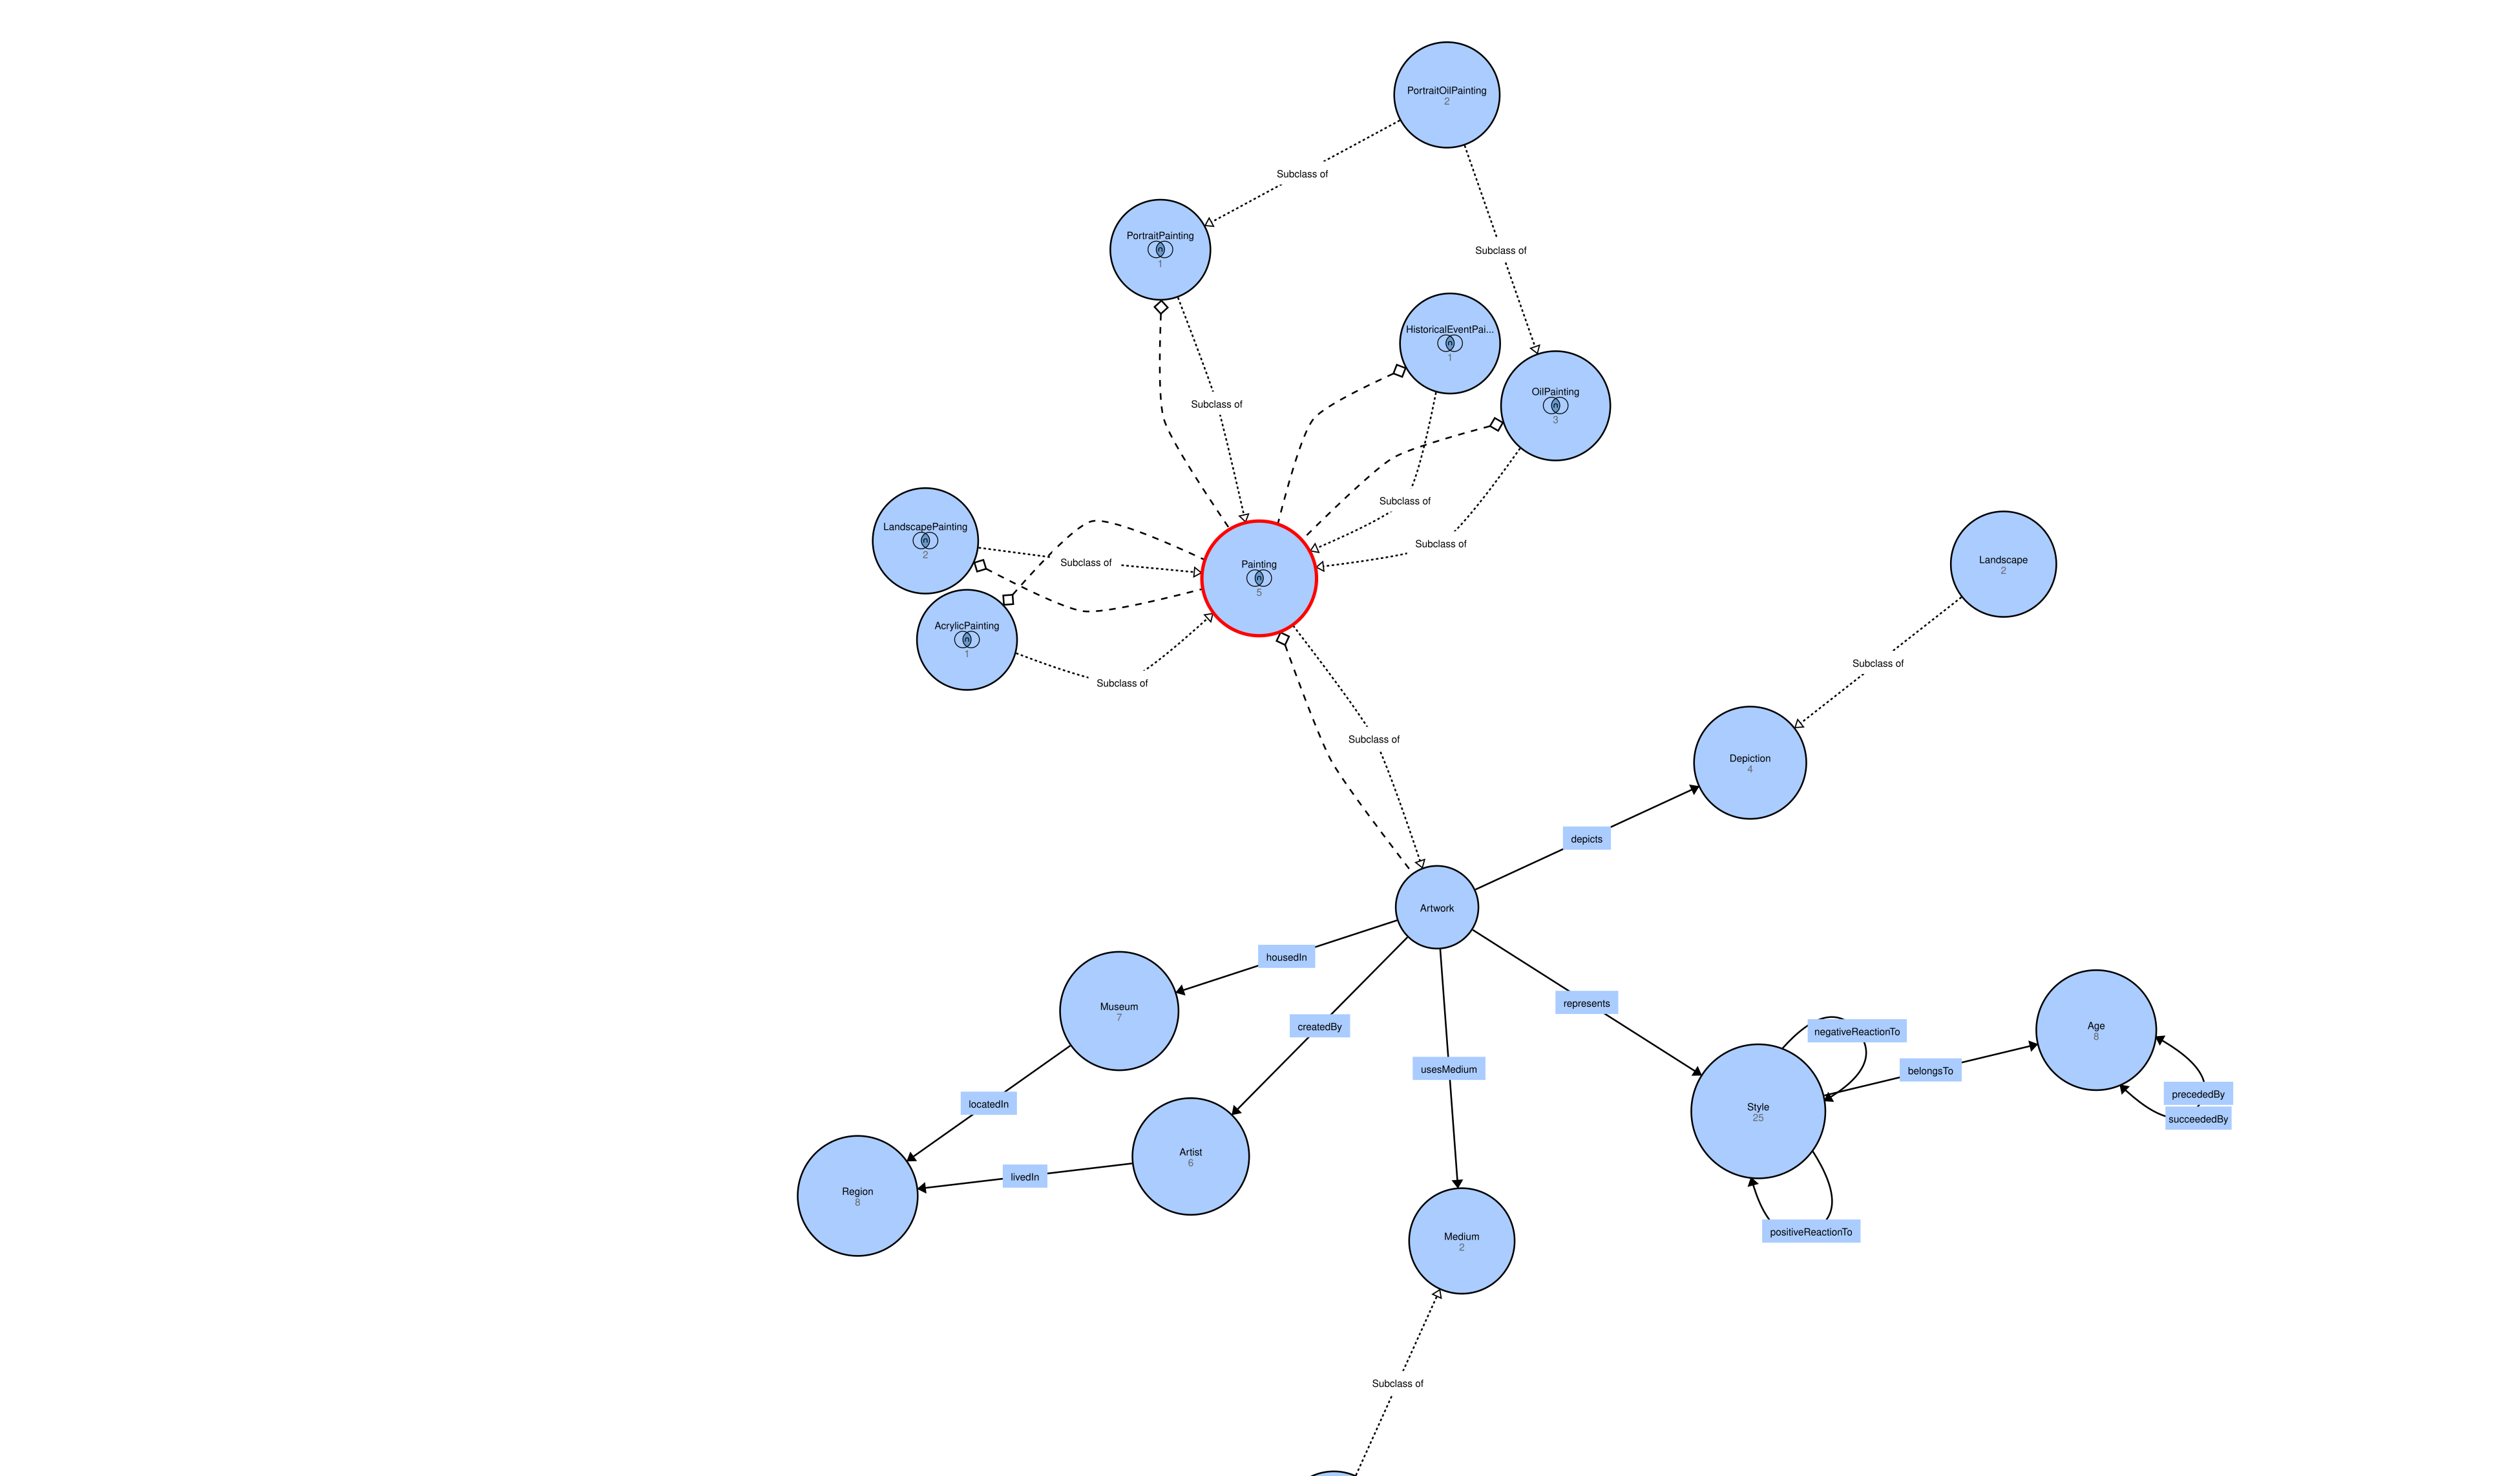
\includegraphics[width=\linewidth]{images/onto.png}  
\end{figure}
\section*{Представители на изброените стилове и епохи}
\subsubsection*{Художници}
\begin{itemize}
  \item $\text{VincentVanGogh} \to \text{Artist}$
    \begin{align*}
      livedIn(VincentVanGogh, WesternEurope)
    \end{align*}
  \item $\text{JohannesVermeer} \to \text{Artist}$
    \begin{align*}
      livedIn(JohannesVermeer, WesternEurope)
    \end{align*}
  \item $\text{LeonardoDaVinci} \to \text{Artist}$
    \begin{align*}
      livedIn(LeonardoDaVinci, WesternEurope)
    \end{align*}
  \item $\text{FranciscoGoya} \to \text{Artist}$
    \begin{align*}
      livedIn(FranciscoGoya, WesternEurope)
    \end{align*}
  \item $\text{AndyWarhol} \to \text{Artist}$
    \begin{align*}
      livedIn(AndyWarhol, NorthAmerica)
    \end{align*}
  \item $\text{ClaudeMonet} \to \text{Artist}$
    \begin{align*}
      livedIn(ClaudeMonet, WesternEurope)
    \end{align*}
\end{itemize}

\subsubsection*{Музеи}
\begin{itemize}
  \item $\text{LouvreMuseum} \to \text{Museum}$
    \begin{align*}
      locatedIn(LouvreMuseum, WesternEurope)
    \end{align*}
  \item $\text{MoMA} \to \text{Museum}$
    \begin{align*}
      locatedIn(MoMA, NorthAmerica)
    \end{align*}
  \item $\text{PradoMuseum} \to \text{Museum}$
    \begin{align*}
      locatedIn(PradoMuseum, WesternEurope)
    \end{align*}
  \item $\text{KatheKollwitzMuseum} \to \text{Museum}$
    \begin{align*}
      locatedIn(KatheKollwitzMuseum, WesternEurope)
    \end{align*}
  \item $\text{BibliotecaRealeTurin} \to \text{Museum}$
    \begin{align*}
      locatedIn(BibliotecaRealeTurin, WesternEurope)
    \end{align*}
  \item $\text{Mauritshuis} \to \text{Museum}$
    \begin{align*}
      locatedIn(Mauritshuis, WesternEurope)
    \end{align*}
\end{itemize}

\subsection*{Картини}
\begin{itemize}
  \item $\text{MonaLisa} \to \text{PortraitPainting, PortraitOilPainting}$
    \begin{figure}[H]
      \centering
      \includegraphics[width=0.25\linewidth]{images/monalisa.jpg}
    \end{figure}
    \begin{align*}
      &createdBy(MonaLisa, LeonardoDaVinci)\\
      &depicts(MonaLisa, Portrait)\\
      &usesMedium(MonaLisa, OilPaint)\\
      &represents(MonaLisa, ItalianRenaissance)\\
      &housedIn(MonaLisa, LouvreMuseum)
    \end{align*}
  \item $\text{PortraitOfAManInRedChalk} \to \text{PortraitPainting}$
    \begin{figure}[H]
      \centering
      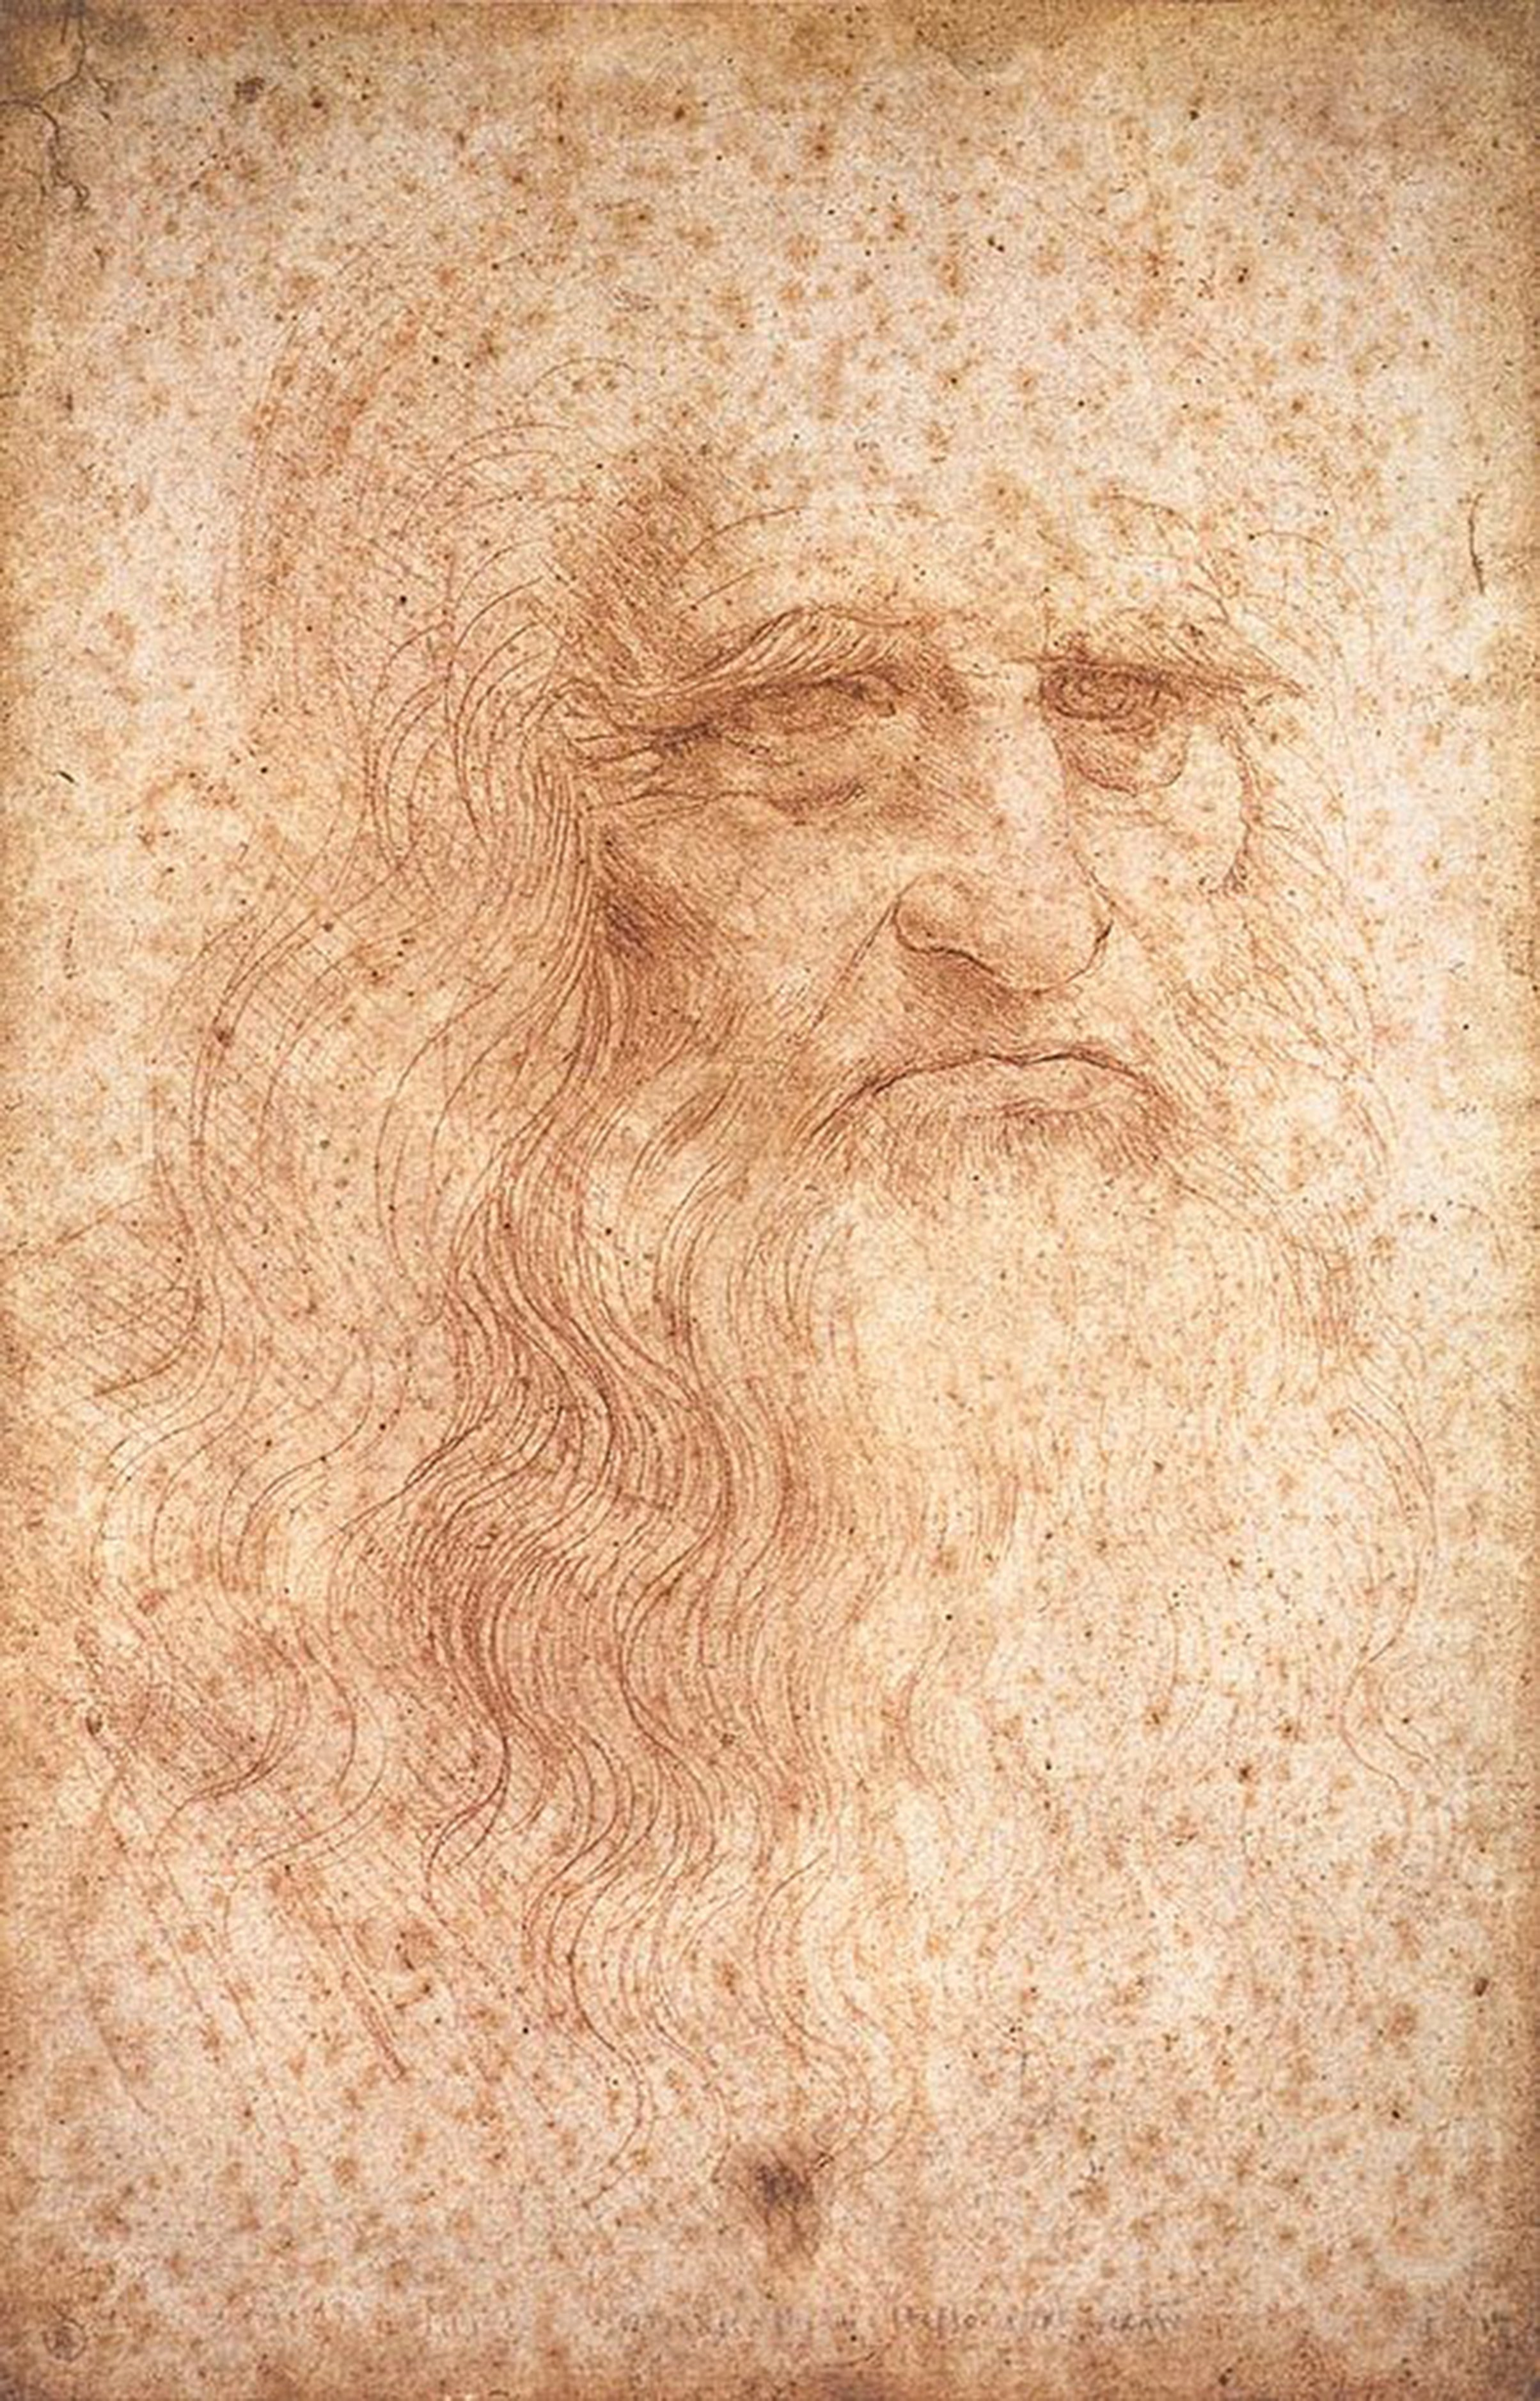
\includegraphics[width=0.35\linewidth]{images/maninredchalk.jpg}
    \end{figure}
    \begin{align*}
      &createdBy(PortraitOfAManInRedChalk, LeonardoDaVinci)\\
      &depicts(PortraitOfAManInRedChalk, Portrait)\\
      &usesMedium(PortraitOfAManInRedChalk, Chalk)\\
      &represents(PortraitOfAManInRedChalk, ItalianRenaissance)\\
      &locatedIn(PortraitOfAManInRedChalk, BibliotecaRealeTurin)
    \end{align*}
  \item $\text{GirlWithAPearlEarring} \to \text{PortraitOilPainting, PortraitPainting}$
    \begin{figure}[H]
      \centering
      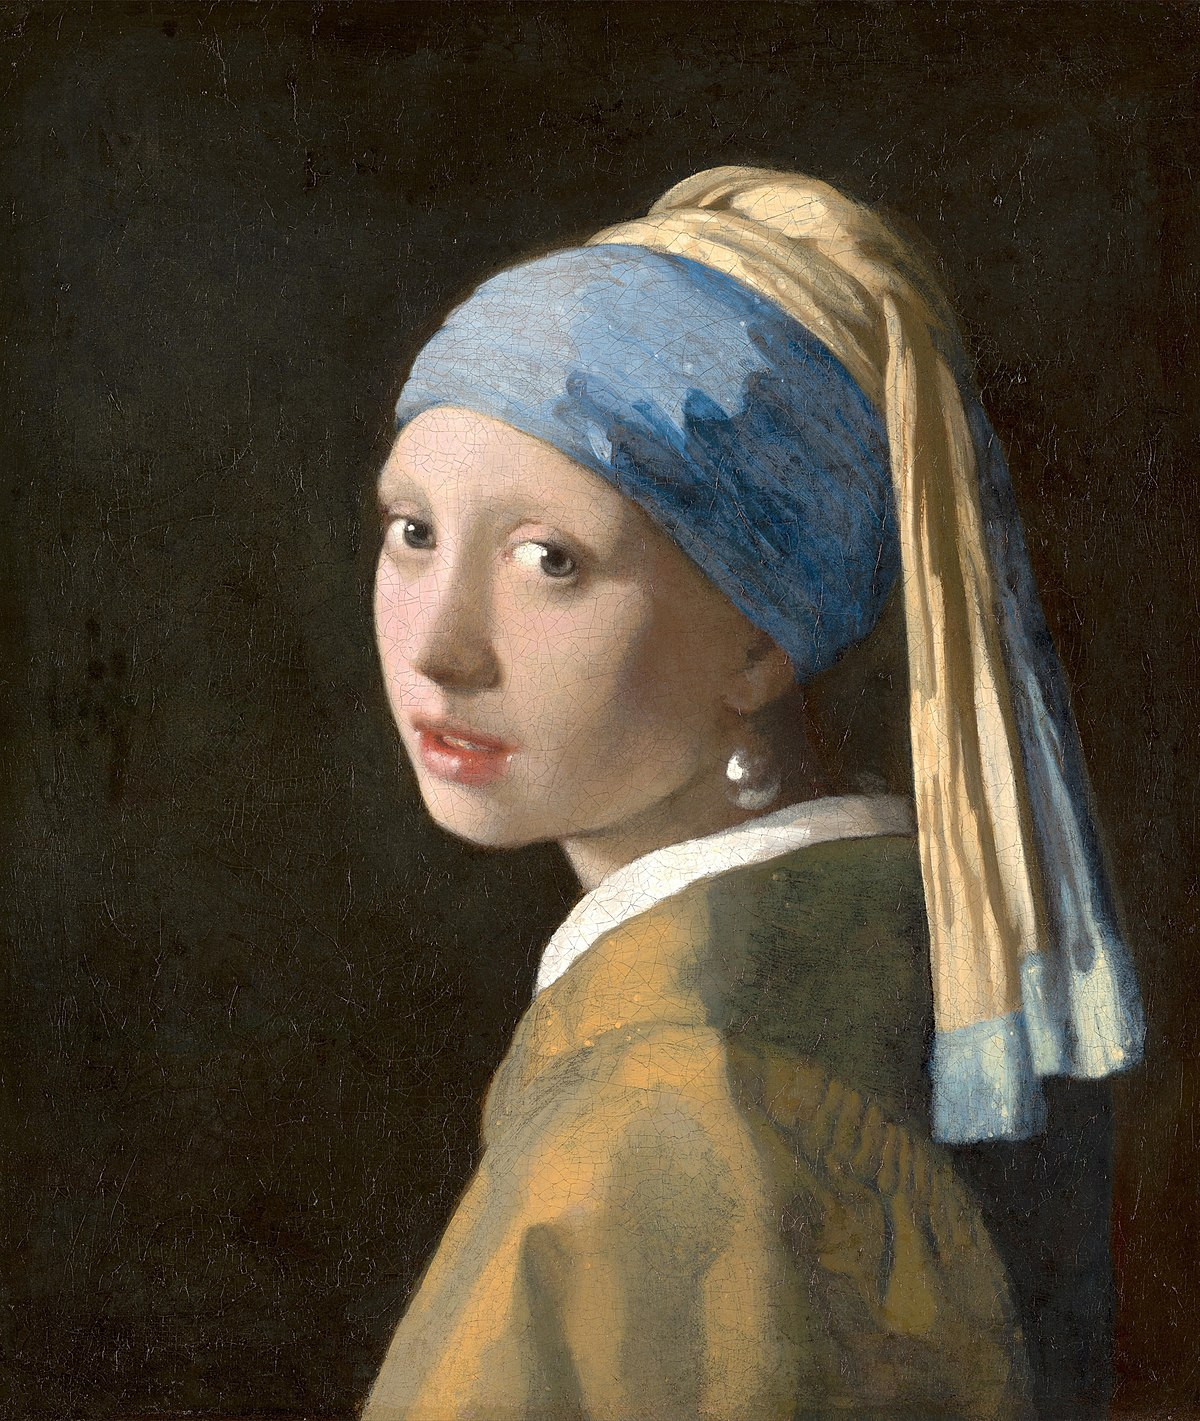
\includegraphics[width=0.35\linewidth]{images/girlwithpearlearring.jpg}
    \end{figure}
    \begin{align*}
      &createdBy(GirlWithAPearlEarring, JohannesVermeer)\\
      &depicts(GirlWithAPearlEarring, Portrait)\\
      &usesMedium(GirlWithAPearlEarring, OilPaint)\\
      &represents(GirlWithAPearlEarring, Baroque)\\
      &housedIn(GirlWithAPearlEarring, Mauritshuis)
    \end{align*}
  \item $\text{CampbellsSoupCans} \to \text{AcrylicPainting}$
    \begin{figure}[H]
      \centering
      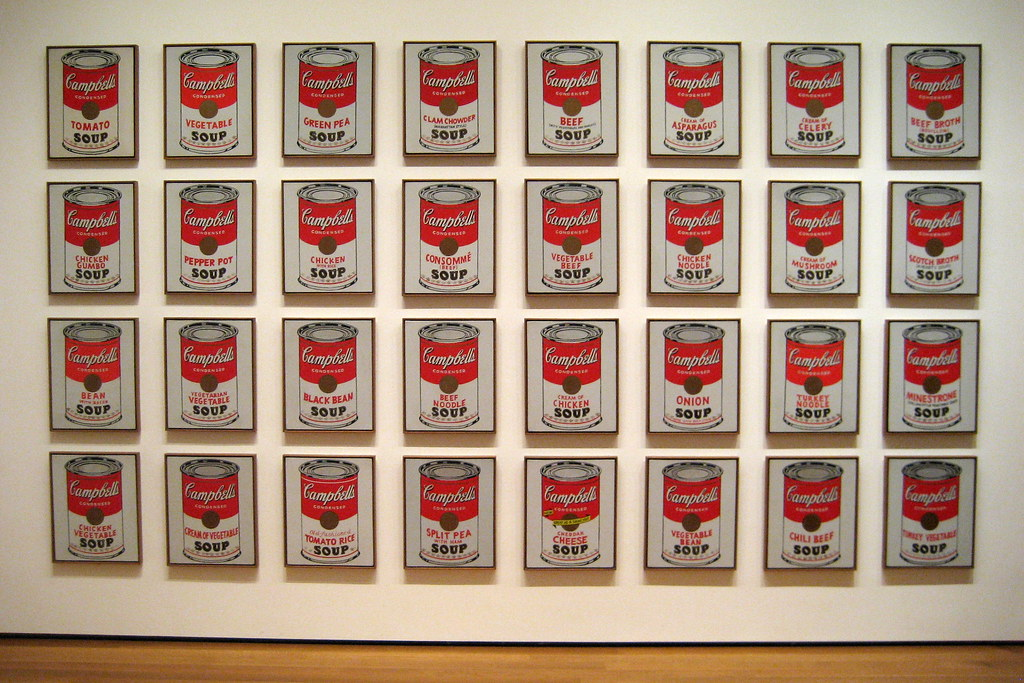
\includegraphics[width=\linewidth]{images/campbellcans.jpg}
    \end{figure}
    \begin{align*}
      &createdBy(CampbellsSoupCans, AndyWarhol)\\
      &depicts(CampbellsSoupCans, AbstractDepiction)\\
      &usesMedium(CampbellsSoupCans, AcrylicPaint)\\
      &represents(CampbellsSoupCans, PopArt)\\
      &housedIn(CampbellsSoupCans, MoMA)\\
      &livedIn(AndyWarhol, NorthAmerica)
    \end{align*}
  \item $\text{ThirdOfMay1808} \to \text{HistoricalEventPainting}$
    \begin{figure}[H]
      \centering
      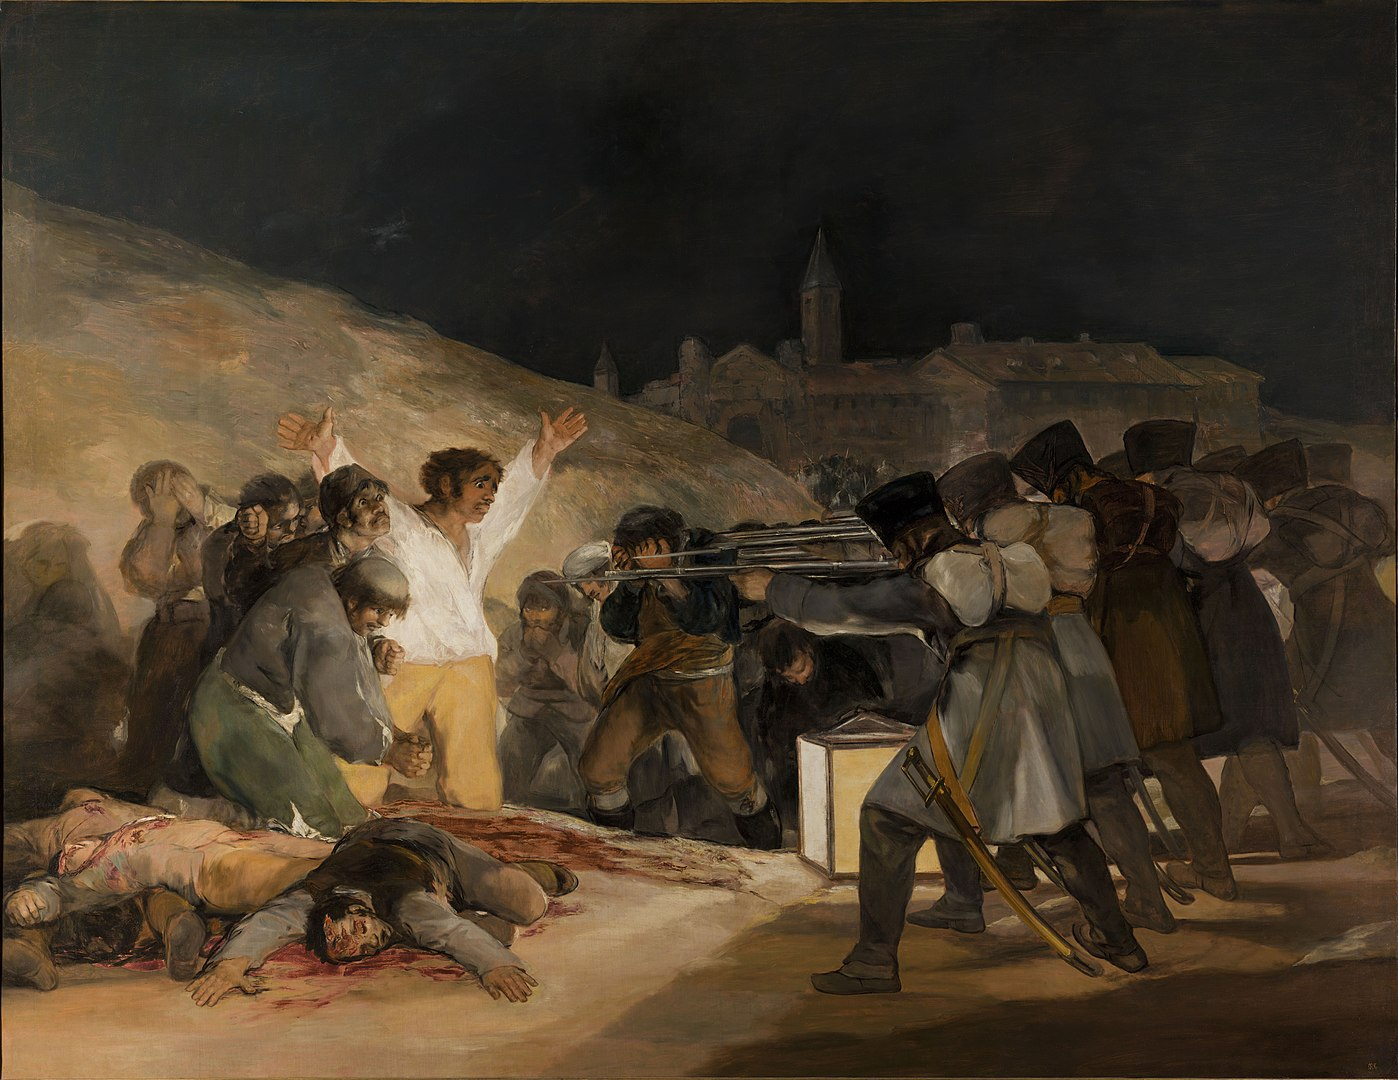
\includegraphics[width=\linewidth]{images/thirdofmay.jpg}
    \end{figure}
    \begin{align*}
      &createdBy(ThirdOfMay1808, FranciscoGoya)\\
      &depicts(ThirdOfMay1808, HistoricalEvent)\\
      &usesMedium(ThirdOfMay1808, OilPaint)\\
      &represents(ThirdOfMay1808, Romanticism)\\
      &housedIn(ThirdOfMay1808, PradoMuseum)
    \end{align*}
  \item $\text{Haystacks} \to \text{LandscapePainting}$
    \begin{figure}[H]
      \centering
      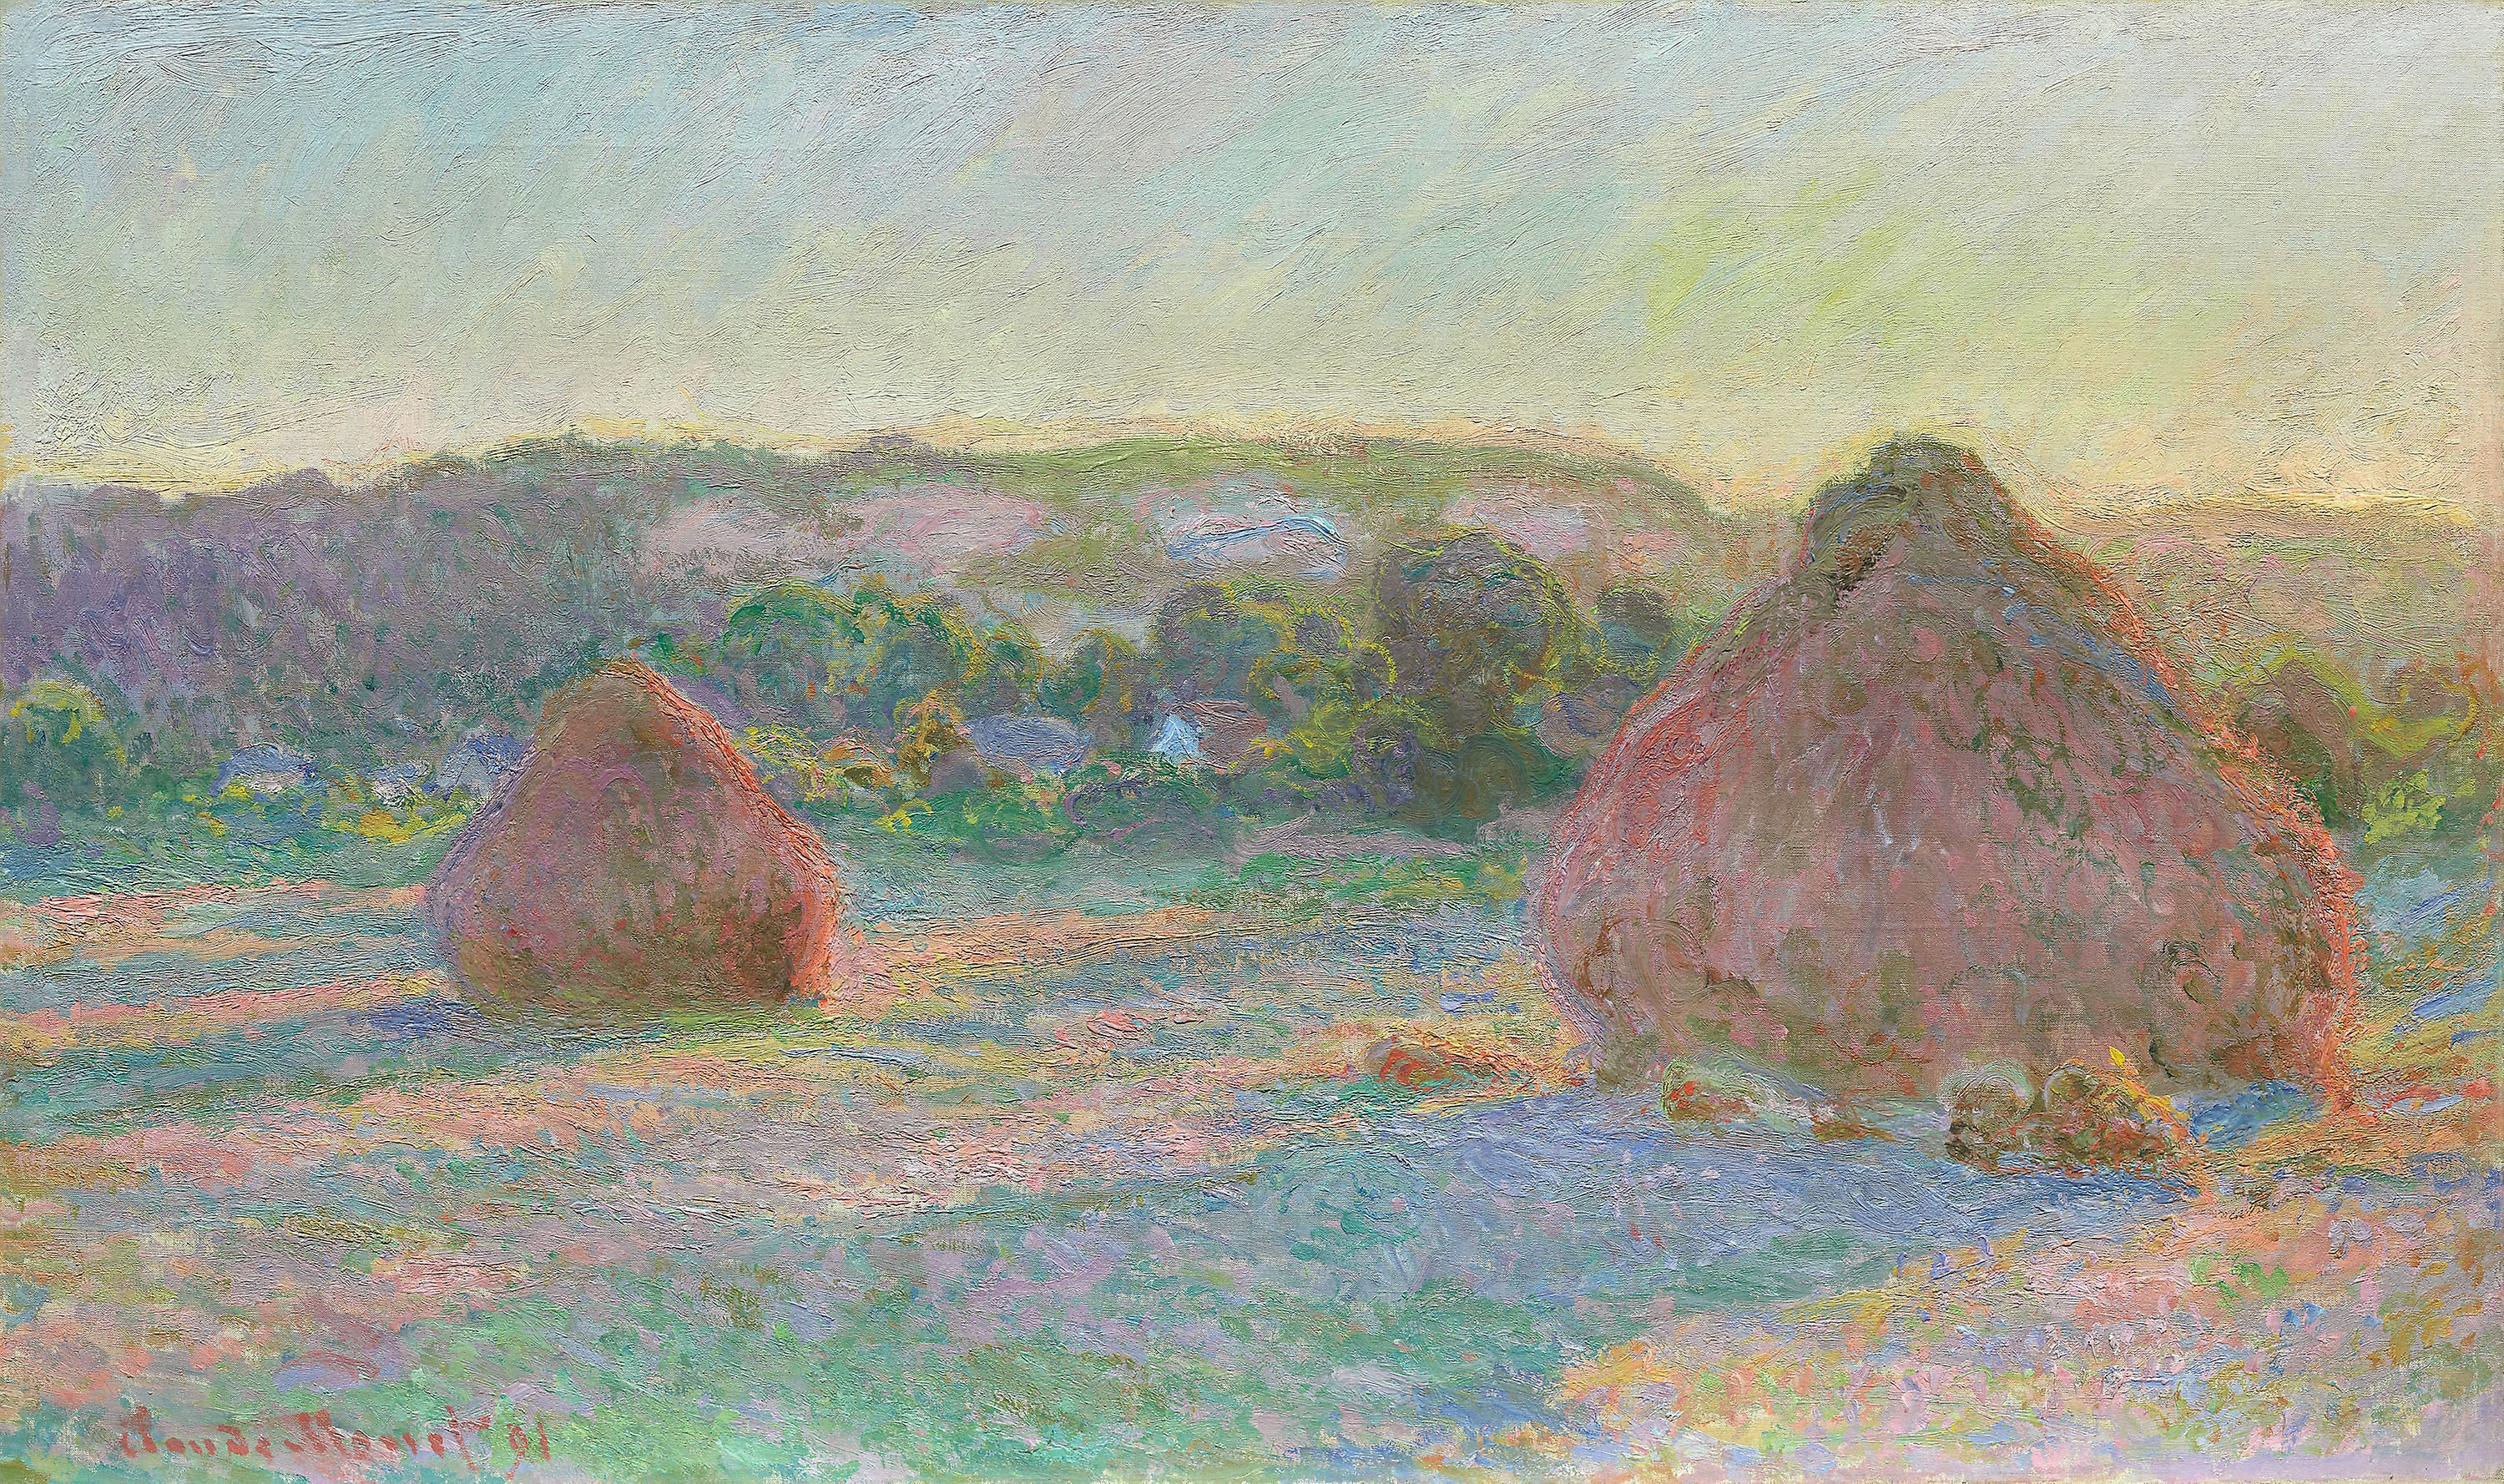
\includegraphics[width=\linewidth]{images/haystacks.jpg}
    \end{figure}
    \begin{align*}
      &\text{createdBy}(\text{Haystacks}, \text{ClaudeMonet})\\
      &\text{housedIn}(\text{Haystacks}, \text{ArtInstituteOfChicago})\\
      &\text{depicts}(\text{Haystacks}, \text{NaturalLandscape})\\
      &\text{represents}(\text{Haystacks}, \text{Impressionism})\\
      &\text{usesMedium}(\text{Haystacks}, \text{OilPaint})
    \end{align*}
  \item $\text{StarryNightOverTheRhone} \to \text{LandscapePainting}$
    \begin{figure}[H]
      \centering
      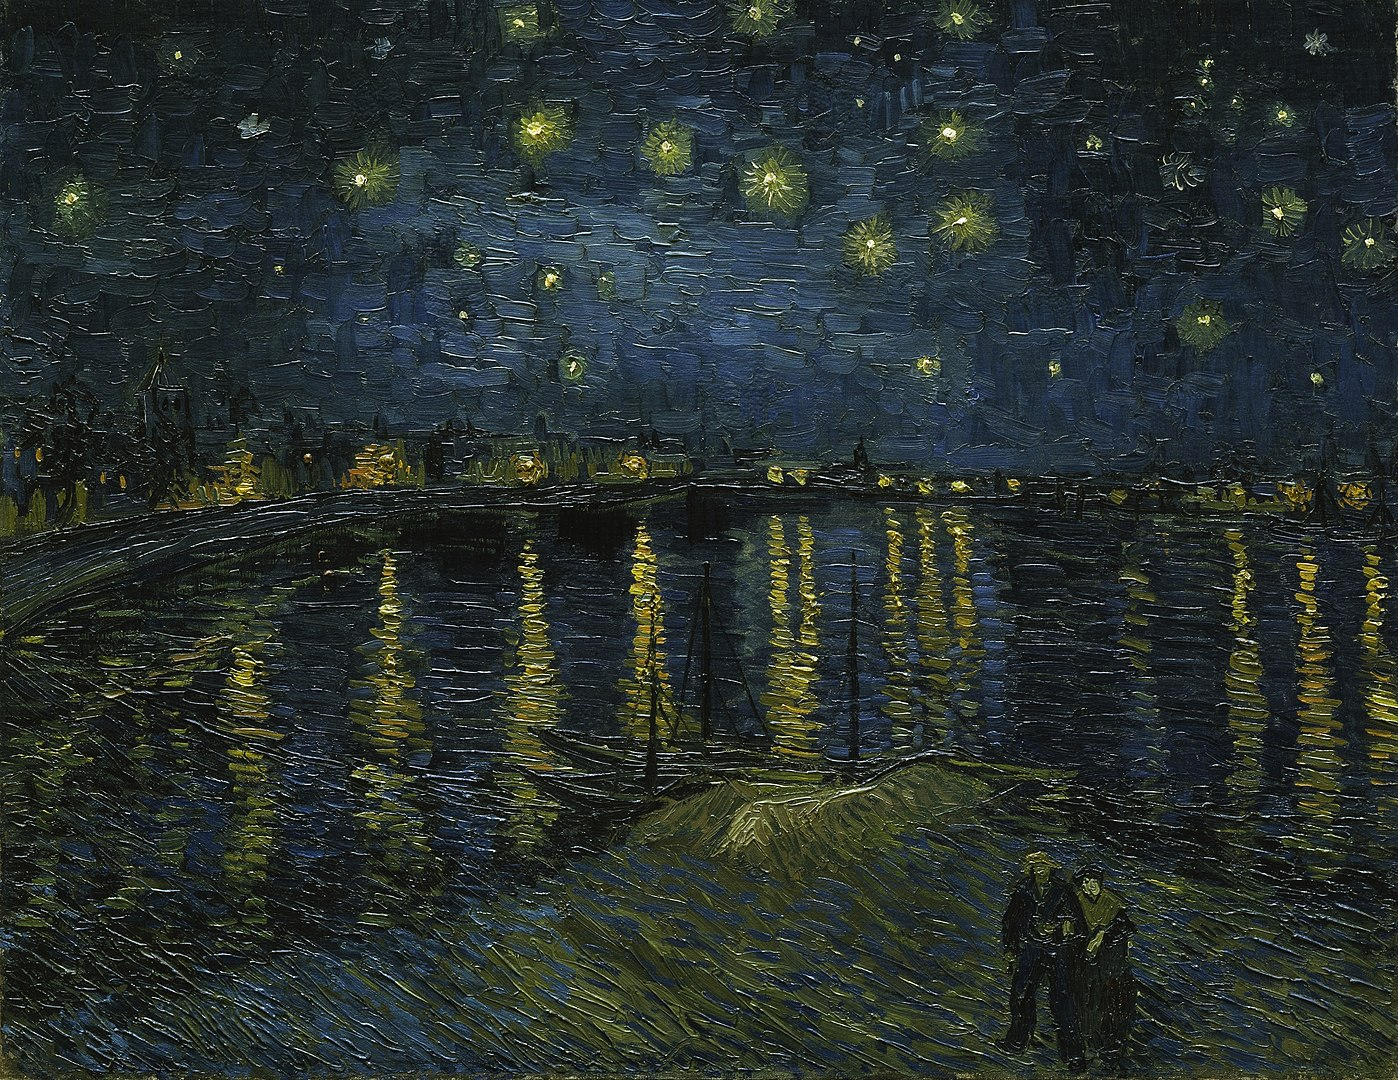
\includegraphics[width=\linewidth]{images/starrynightovertherhone.jpg}
    \end{figure}
    \begin{align*}
      &createdBy(StarryNightOverTheRhone, VincentVanGogh)\\
      &depicts(StarryNightOverTheRhone, NaturalLandscape)\\
      &usesMedium(StarryNightOverTheRhone, OilPaint)\\
      &represents(StarryNightOverTheRhone, PostImpressionism)\\
      &housedIn(StarryNightOverTheRhone, MoMA)
    \end{align*}
\end{itemize}
\section*{Заявки}
Примерните заявки по-долу могат да бъдат изразени чрез разширение на езика $\mathcal{DL}$, което поддържа променливи и отрицания\cite{halReasoningDescription}.
\begin{itemize}
  \item Да се намери всяка картина, която е изложени в музей, разположен  в регион, различен от този, където е живял художникът ѝ
    \begin{align*}
      \text{MovedPainting } \doteq
      &\text{Painting } \sqcap\\
      &\exists \text{ createdBy}.(\text{Artist }\sqcap \exists \text{ :livedIn}.\text{?artistRegion}) \sqcap\\
      &\exists \neg(\text{ housedIn}.(\text{Museum} \sqcap \exists \text{ :locatedIn}.\text{?artistRegion}))
    \end{align*}
  \item Да се намерят тези художници, които са изработили портрети с различни графични средства
    \begin{align*}
      \text{PortraitMaster } \doteq\\
      &\text{Artist } \sqcap \\
      &\exists \text{ :createdBy}.(\text{Artwork} \sqcap \exists \text{ :depicts}.\text{Portrait} \sqcap \exists \text{ :usesMedium}.\text{?medium1}) \sqcap \\
      &\exists \text{ :createdBy}.(\text{Artwork} \sqcap \exists \text{ :depicts}.\text{Portrait} \sqcap \exists\neg (\text{:usesMedium}.\text{?medium2}))
    \end{align*}
\end{itemize}
Синтаксисът на Protege не позволява променливи, но заявките могат да бъдат изразени чрез SPARQL по следния начин:
\begin{lstlisting}[language=SPARQL]
  PREFIX rdf: <http://www.w3.org/1999/02/22-rdf-syntax-ns#>
  PREFIX owl: <http://www.w3.org/2002/07/owl#>
  PREFIX rdfs: <http://www.w3.org/2000/01/rdf-schema#>
  PREFIX xsd: <http://www.w3.org/2001/XMLSchema#>
  PREFIX : <http://example.org/art_ontology.owl#>

  SELECT DISTINCT ?painting
  WHERE {
    ?painting rdf:type/rdfs:subClassOf* :Painting .
    ?painting :createdBy ?artist .
    ?painting :housedIn ?museum .
    ?artist :livedIn ?artistRegion .
    ?museum :locatedIn ?museumRegion .
    FILTER (?artistRegion != ?museumRegion)
  }

  SELECT DISTINCT ?artist
  WHERE {
    ?painting1 :depicts :Portrait .
    ?painting1 :createdBy ?artist .
    ?painting1 :usesMedium ?medium .

    ?painting2 :depicts :Portrait .
    ?painting2 :createdBy ?artist .
    ?painting2 :usesMedium ?otherMedium .
    FILTER (?medium != ?otherMedium)
  }
\end{lstlisting}
\section*{Сравнение с други онтологии}
Кратко търсене в интернет откри много ограничено множество онтологии на естествен език, които са посветени на изкуството, сред които най-популярна е тази на Oxford\cite{Davies2009-hf}. Опит за достъп на 14.12.2024 чрез университетския ми профил върна грешка. 
\newline
Търсенето обаче не откри онтологии, които са машинно четими. Затова ще посоча някои предимства, недостатъци и възможности за подобрения, които не са базиран на съпоставка с други онтологии:
\begin{itemize}
  \item онтологията е консистентна
  \item зададени са подходящ брой ограничения над ролите, които да помогнат в логическите изводи, но да не намалят изразителната сила на онтологията - например ролята \emph{represents} не е функционална, което отразява възможността едно произведение на изкуството да е екземпляр на повече от един стил
  \item онтологията е проектирана да подлежи на лесно разширение:
  \begin{itemize}
    \item за различни видове техники - може да бъдат добавени концепти като \emph{Technique}
    \item за всякакви видове изкуство чрез общия концепт \emph{Artwork}, който може да бъде разширен не само с \emph{Painting}, но и други видове творби - например скулптури, чрез \emph{Sculpture} чрез допълнителни ограничения с други концепти, например \emph{Medium}, към който може да бъдат добавени константи или подконцепти като \emph{HardMaterial, Marble} и др.
  \end{itemize}
  \item могат да бъдат дефинирани роли, задаващи точни години за началото и края на епохите, които, с подходящи правила за извод, могат да заменят релациите \emph{precededBy} и \emph{succeededBy}. По този начин епохите могат да се застъпват. Тази онтология умишлено не беше проектирана така с цел да бъдат спазени изискванията за брой и вид на ролите.
  \item съществуват десетки други стилове и хиляди произведения на изкуството, които не фигурират в онтологията и могат да бъдат добавени след консултация с експерт в областта. 
\end{itemize}
\nocite{wikipediaCampbellsSoup,wikipediaGirlWith,wikipediaMonaLisa,wikipediaPortraitChalk,wikipediaThird1808,wikipediaHaystacksMonet,wikipediaStarryNight,wikipediaPeriodsWestern,wikipediaVisualArts,studiobinderHistoryTimeline}
\printbibliography

\end{document}
